\begin{frame}{Aggregation Operations (1)}
  \begin{itemize}
      \item Aggregations process data records and return computed results
      \item in mongodb there are three types of aggregations
      \begin{itemize}
        \item Single Purpose Aggregation Operations
        \item Map-Reduce
        \item Aggregation Pipelines
      \end{itemize}
      \item we will only talk about these briefly
  \end{itemize}
\end{frame}

\begin{frame}{Aggregation Operations (2): Single Purpose Aggregation Operations}
  \begin{itemize}
    \item \lstinline[basicstyle=\ttfamily]{db.my\_collection.count(query)}
      \inote{Count the number of documents that match}
    \item \lstinline[basicstyle=\ttfamily]{db.my\_collection.distinct(field)}
      \inote{return an array of the distinct values of the field}
    \item \lstinline[basicstyle=\ttfamily]{db.my\_collection.group(query)}
      \inote{groups documents, supports aggregation-pipeline like operations}
    \end{itemize}
\end{frame}

\begin{frame}{Aggregation Operations (3): Map-Reduce}
  \begin{itemize}
    \item is a general data processing paradigm
      \inote{filter \& sort data using Map, then summarise it Reduce}
  \end{itemize}
  \begin{center}
    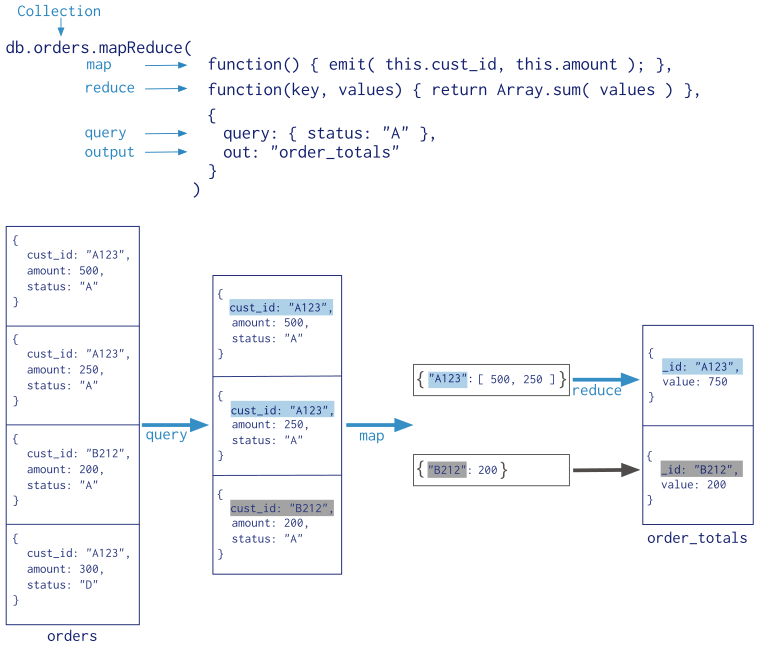
\includegraphics[width=0.8\textheight]{imgs/map-reduce.png}
  \end{center}
\end{frame}

\begin{frame}{Aggregation Operations (5): Aggregation Pipeline}
  \begin{itemize}
    \item modeled on the concept of data processing pipelines
      \inote{multi-stage pipeline as an alternative to Map-Reduce}
  \end{itemize}
  \begin{center}
    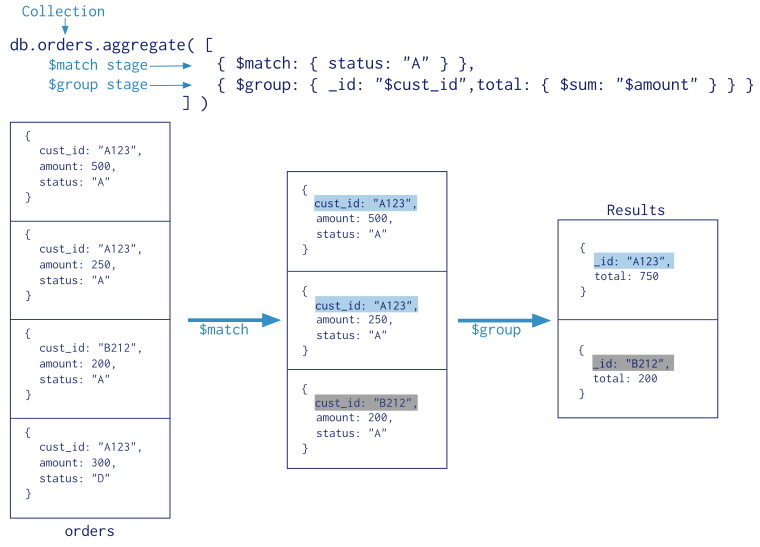
\includegraphics[width=0.8\textheight]{imgs/aggregation-pipeline.png}
  \end{center}
\end{frame}
